% !TEX root = ../main.tex
\pagebreak
\lecture{2}{2026-09-24}{Woche 2 Grunlagen Management II}
\url{https://lms.uzh.ch/auth/RepositoryEntry/17910989063/CourseNode/102309852135373/path%3D~~VL%20II%20%2D%2024%2E09%2E2026/0}
\section{Funktionen des Managements}
\subsection{Institutioneller \& funktionaler Managementbegriff}
\begin{itemize}
    \item \textbf{Institutionelles Begriffsverstaendnis}
    \subitem Gruppe von Personen einer Org die über Führungs und Weisungsbefugnis verfügen
    \subitem für steuerung 
    \item \textbf{Funktionales}
    \subitem Bündel Funktionen
    \subitem Rollen oder Funktionen nötig für die Steuerung  
\end{itemize}

\subsubsection{Klasische Funktionen und Prozesse}
\begin{enumerate}
    \item Planung (\textbf{Primär} gestaltende Voraussetzung) 
    \subitem Zielen, Richtilinien
    \item Organisation
    \subitem  Plangerechter Einheiten
    \subitem Zuweisung Kompentenzen
    \item Personaleinsatz
        \subitem Nach Anforderung passende Auswahl von Personal, Lohn, Entwicklung 
    \item Fuehrung
        \subitem Arbeiter Korrektur und Belohnung nach Ziel 
    \item Kontrolle
    \item wiederum Planung (Zyklus neugestartet)
\end{enumerate}
\footnote{Scheint linear aber praktisch auch paralell }
\pagebreak
\subsection{Planung}
Durch Planung werden die weiteren Funktionen gestaltet
\begin{itemize}
    \item Art der Organisation
    \item Personal Auswahl
    \item Fuehrungsart
    \item Bestimmung der Kontrollstandards
\end{itemize}

\subsubsection{Planung vs Realitaet}
Annahmen bei der Planung, ist die Durchschaubarkeit der Unternehmensprozesse. In Realität sind Prozesse vielseitig und komplex.
\begin{theorem}
    \textbf{Daher sollten Managementfunktionen multipersonal und dezentral vollzogen werden.}
\end{theorem}

\section{Reformvorschlag: Strategischer Managementprozess}
\textbf{Drei Ebenen}
\begin{itemize}
    \item Strategisches Management
    \subitem Strategische nur Planung und Kontrolle (Wettbewerbsstrategie, Produkt.Markt.Kozept)
    \subitem Metaplanung (planung des Strategischen managements)
    \item Operatives
        \subitem Umsetzung des Geplanten
    \item Effiziente Umsetyung der strategischen Zielen und Pläne
\end{itemize}

\pagebreak
\textbf{Zeitsynchrone Interdependenz der drei Ebenen}

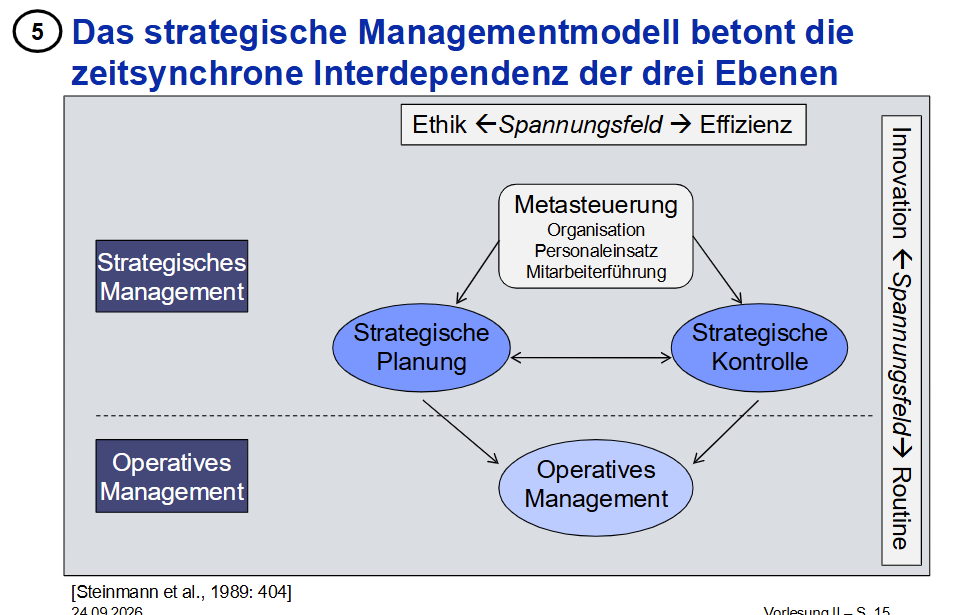
\includegraphics[width=\textwidth,height=0.7\textheight,keepaspectratio]{figures/Drei_Ebenen.png}


Alle Mitglieder der Organisation, tragen zur strategischen Steuerung bei.

\subsection{Die Zweispannungsfelder}

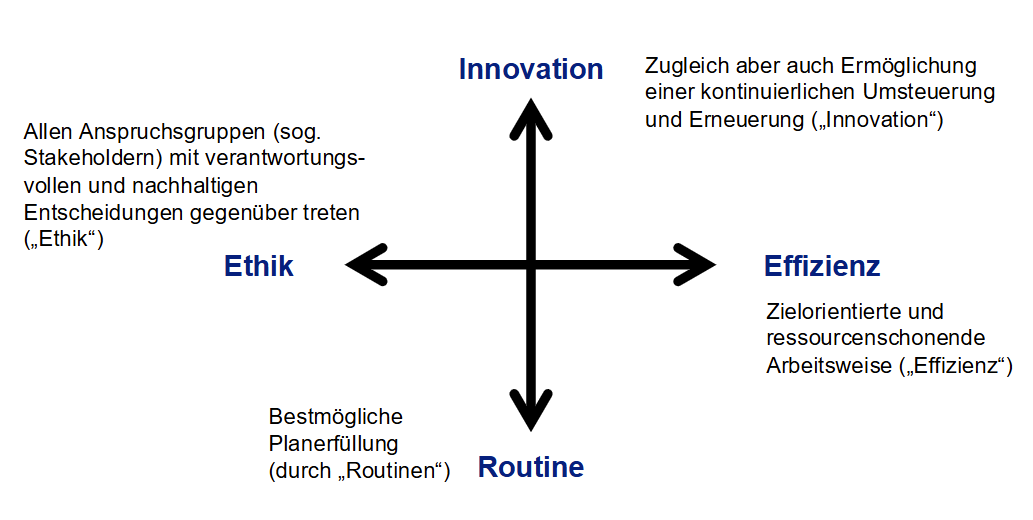
\includegraphics[width=\textwidth,height=0.7\textheight,keepaspectratio]{figures/Spannungsfelder.png}


\pagebreak
\subsection{Five Forces - Wettbewerbskräfte}
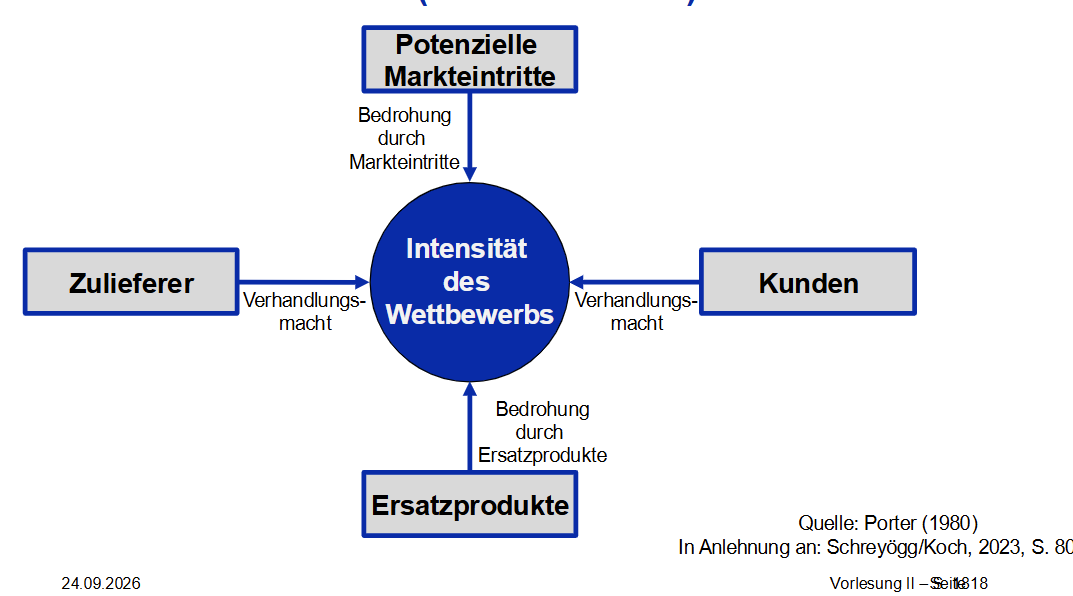
\includegraphics[width=\textwidth,height=0.7\textheight,keepaspectratio]{figures/FiveForces.png}
Leiten sich aus bedingungen eines perfekten Marktes ab. \footnote{SchreyoeggKoch S.80}
